 \documentclass[12pt, oneside]{article}

\usepackage[letterpaper, scale=0.89, centering]{geometry}
\usepackage{fancyhdr}
\setlength{\parindent}{0em}
\setlength{\parskip}{1em}

\pagestyle{fancy}
\fancyhf{}
\renewcommand{\headrulewidth}{0pt}
\rfoot{\href{https://creativecommons.org/licenses/by-nc-sa/2.0/}{CC BY-NC-SA 2.0} Version \today~(\thepage)}

\usepackage{amssymb,amsmath,pifont,amsfonts,comment,enumerate,enumitem}
\usepackage{currfile,xstring,hyperref,tabularx,graphicx,wasysym}
\usepackage[labelformat=empty]{caption}
\usepackage[dvipsnames,table]{xcolor}
\usepackage{multicol,multirow,array,listings,tabularx,lastpage,textcomp,booktabs}

\lstnewenvironment{algorithm}[1][] {   
    \lstset{ mathescape=true,
        frame=tB,
        numbers=left, 
        numberstyle=\tiny,
        basicstyle=\rmfamily\scriptsize, 
        keywordstyle=\color{black}\bfseries,
        keywords={,procedure, div, for, to, input, output, return, datatype, function, in, if, else, foreach, while, begin, end, }
        numbers=left,
        xleftmargin=.04\textwidth,
        #1
    }
}
{}
\lstnewenvironment{java}[1][]
{   
    \lstset{
        language=java,
        mathescape=true,
        frame=tB,
        numbers=left, 
        numberstyle=\tiny,
        basicstyle=\ttfamily\scriptsize, 
        keywordstyle=\color{black}\bfseries,
        keywords={, int, double, for, return, if, else, while, }
        numbers=left,
        xleftmargin=.04\textwidth,
        #1
    }
}
{}

\newcommand\abs[1]{\lvert~#1~\rvert}
\newcommand{\st}{\mid}

\newcommand{\A}[0]{\texttt{A}}
\newcommand{\C}[0]{\texttt{C}}
\newcommand{\G}[0]{\texttt{G}}
\newcommand{\U}[0]{\texttt{U}}

\newcommand{\cmark}{\ding{51}}
\newcommand{\xmark}{\ding{55}}

 
\begin{document}
        
        
        \fbox{\parbox{\textwidth}{%
{\bf New!} An algorithm is a finite sequence of precise instructions for solving a problem.
\hfill
}}
A relation $R$ on a set $A$ is called {\bf antisymmetric} means 
$\forall a \in A ~\forall b \in A~\left(~\left( ~(a,b) \in R \land (b,a) \in R ~\right) \to a=b~\right)$

{\bf Definition} For $b$ an integer greater than $1$ and $n$ a positive integer, 
the {\bf base $b$ expansion of $n$}  is
\[
(a_{k-1} \cdots a_1 a_0)_b
\]
where $k$ is a positive integer, $a_0, a_1, \ldots, a_{k-1}$ 
are nonnegative integers less than $b$, $a_{k-1} \neq  0$, and
\[
n =  \sum_{i=0}^{k-1} a_{i} b^{i}
\]
Notice: {\it The base $b$ expansion of a positive integer $n$ is a string over the alphabet 
$\{x \in \mathbb{N} \st x < b\}$
whose leftmost character is nonzero.}
\begin{center}
\begin{tabular}{|c|c|}
\hline
Base $b$ & Collection of possible coefficients in base $b$ expansion of  a positive integer \\
\hline
& \\
Binary ($b=2$) & $\{0,1\}$ \\
\hline
& \\
Ternary ($b=3$) & $\{0,1, 2\}$ \\
\hline
& \\
Octal ($b=8$) & $\{0,1, 2, 3, 4, 5, 6, 7\}$\\
\hline
& \\
Decimal ($b=10$) & $\{0,1, 2, 3, 4, 5, 6, 7, 8, 9\}$\\
\hline
& \\
Hexadecimal ($b=16$) &  $\{0,1, 2, 3, 4, 5, 6, 7, 8, 9, A, B, C, D, E, F\}$\\
& letter coefficient symbols represent numerical values $(A)_{16} = (10)_{10}$\\
&$(B)_{16} = (11)_{10} ~~(C)_{16} = (12)_{10} ~~
 (D)_{16} = (13)_{10} ~~ (E)_{16} = (14)_{10} ~~ (F)_{16} = (15)_{10} $\\
\hline
\end{tabular}
\end{center}

{\bf Definition} : A function $f: D  \to C$ is a {\bf bijection} means that it is both 
one-to-one  and onto. The {\bf inverse} of a  bijection $f: D  \to  C$ is 
the function $g: C  \to  D$  such that $g(b) = a$ iff  $f(a) =  b$.

{\bf Definition}: When $A$ and $B$ are sets, we say any subset of $A \times B$ is a {\bf binary relation}. 
A relation $R$ can also be represented as
\begin{itemize}
\item A function $f_{TF} : A \times B \to \{T, F\}$
where, for $a \in A$ and $b \in B$, $f_{TF}(~(a,b)~) = 
\begin{cases} 
    T \qquad&\text{when } (a,b) \in R \\
    F \qquad&\text{when } (a,b) \notin R
\end{cases}$
\item A function $f_{\mathcal{P}} : A   \to \mathcal{P}(B)$ where, for $a \in A$, 
$f_{\mathcal{P}}( a ) = \{ b \in B ~|~ (a,b) \in R \}$
\end{itemize}
When $A$ is a set, we say any subset of $A \times A$ is a (binary) {\bf relation} on $A$.

For nonempty sets $A, B$ we say
\begin{align*}
|A| \leq |B| &\text{ means there is a one-to-one function with domain $A$, codomain $B$} \\
|A| \geq |B| &\text{ means there is an onto function with domain $A$, codomain $B$} \\
|A| = |B| &\text{ means there is a bijection with domain $A$, codomain $B$}
\end{align*}
For all sets $A$, we say $|A| = |\emptyset|$, $|\emptyset| = |A|$ if and only if $A = \emptyset$.
{\bf Definition}:  For nonempty sets $A, B$, we say that {\bf the  cardinality of $A$ is  no  bigger than the cardinality of $B$}, 
and write $|A| \leq |B|$, to mean there is a  one-to-one function  with domain $A$  and codomain $B$.
Also, we define $|\emptyset| \leq |B|$ for all sets $B$.
{\bf Definition}:  For nonempty sets $A, B$, we say that {\bf the  cardinality of $A$ is  no  smaller than 
the cardinality of  $B$}, and 
write $|A| \geq |B|$, to mean there is an onto function  with domain $A$  and codomain $B$.
Also, we define $|A| \geq |\emptyset|$ for all sets $A$.

{\bf Definition}: The {\bf Cartesian product} of the sets $A$ and $B$, 
$A \times B$, is the set of all ordered pairs $(a, b)$, where $a \in A$ and $b \in B$. 
That is: $A \times B = \{(a, b) \mid (a \in A) \land (b \in B)\}$.
The Cartesian product of the sets $A_1, A_2, \ldots ,A_n$, denoted by 
$A_1 \times A_2 \times \cdots \times A_n$, is the
set of ordered n-tuples $(a_1, a_2,...,a_n)$, where $a_i$ belongs to 
$A_i$ for $i = 1, 2,\ldots,n$. That is,
\[
    A_1 \times A_2 \times \cdots \times A_n = \{(a_1, a_2,\ldots,a_n) \mid a_i \in A_i \textrm{ for } i = 1, 2,\ldots,n\}
\]
{\bf Proposition}: Declarative sentence that is true or false (not both).
{\bf Propositional variable}: Variable that represents a proposition.
{\bf Compound proposition}: New proposition formed from existing propositions (potentially) using logical operators.
{\it Note}: A propositional variable is one example of a compound proposition.
{\bf Truth table}: Table with one row for each of the possible combinations of truth values of the input and 
    an additional column that shows the truth value of the result of the operation corresponding to a particular row.
    

We can use a recursive definition to describe all 
compound propositions that use propositional variables 
from a specified collection.  Here's the definition
for all compound propositions whose propositional variables 
are in $\{p, q\}$.
\[
\begin{array}{ll}
\textrm{Basis Step: } & p \textrm{ and } q \textrm{ are each a compound proposition} \\
\textrm{Recursive Step: } & \textrm{If } x \textrm{ is a compound proposition then so is } (\lnot x) 
\textrm{ and if } \\
& x \textrm{ and } y \textrm{ are both compound propositions then so is each of }\\
&(x \land y), (x \oplus y), (x \lor y), (x \to y), (x \leftrightarrow y)
\end{array}
\]
{\bf Definition}: A set $A$ is {\bf countably infinite} means it is the 
same size as $\mathbb{N}$.

\begin{center}
\begin{tabular}{|llp{9.8cm}|}
\hline
{\bf Term} & {\bf Notation Example(s)} & {\bf We say in English \ldots } \\
\hline
%$n$-tuple & $(x_1, x_2, x_3)$ & The 3-tuple of $x_1$, $x_2$, and $x_3$ \\
%          & $(3, 4)$ & The 2-tuple or {\bf ordered pair} of $3$ and $4$ \\
sequence & $x_1, \ldots, x_n$ & A sequence $x_1$ to $x_n$ \\
%         & $x_1, \ldots, x_n$ where $n = 0$ & An empty sequence \\
%         & $x_1, \ldots, x_n$ where $n = 1$ & A sequence containing just $x_1$ \\
%         & $x_1, \ldots, x_n$ where $n = 2$ & A sequence containing just $x_1$ and $x_2$ in order \\
%         & $x_1, x_2$ & A sequence containing just $x_1$ and $x_2$ in order \\
summation & $\sum_{i=1}^n x_i$ or $\displaystyle{\sum_{i=1}^n x_i}$ & The sum of the terms of the sequence $x_1$ to $x_n$ \\
&&\\
%maximum & $\displaystyle \max(x, y)$ & The max of $x$ and $y$, when they are numbers \\ % Note that this is different than summation!
%        & $\displaystyle \max_{1 \leq i \leq n} x_i$ & The max of $x_1$ to $x_n$, when they are numbers \\ % Also different from display
%&&\\
%set & & Unordered collection of objects. The set of \ldots \\
all reals & $\mathbb{R}$ & The (set of all) real numbers (numbers on the number line)\\
all integers & $\mathbb{Z}$ & The (set of all) integers (whole numbers including negatives, zero, and positives) \\
all positive integers & $\mathbb{Z}^+$ & The (set of all) strictly positive integers \\
all natural numbers & $\mathbb{N}$ & The (set of all) natural numbers. {\bf Note}: we use the convention that $0$ is a natural number. \\
%roster method & $\{43, 7, 9\}$ & The set whose elements are $43$, $7$, and $9$\\
%              & $\{9, \mathbb{N}\}$ & The set whose elements are $9$ and $\mathbb{N}$\\
%&&\\
%set builder notation & $\{ x \in \mathbb{Z} \mid x > 0\}$ & The set of all $x$ from the integers such that $x$ is greater than $0$ \\
%                     & $\{ 3x  \mid x \in \mathbb{Z} \}$ & The set of all integer multiples of $3$. {\bf Note}: we use the convention that writing two numbers next to each other means multiplication. \\
&&\\
%function rule definition & $f(x) = x + 4$ & Define $f$ of $x$ to be $x + 4$ \\
piecewise rule definition & $f(x) = \begin{cases} x & \text{if~}x \geq 0 \\ -x & \text{if~}x<0\end{cases}$ &
Define $f$ of $x$ to be $x$ when $x$ is nonnegative and to be $-x$ when $x$ is negative\\
function application & $f(7)$ & $f$ of $7$ {\bf or} $f$ applied to $7$ {\bf or} the image of $7$ under $f$\\
                     & $f(z)$ & $f$ of $z$ {\bf or} $f$ applied to $z$ {\bf or} the image of $z$ under $f$\\
                     & $f(g(z))$ & $f$ of $g$ of $z$ {\bf or} $f$ applied to the result of $g$ applied to $z$ \\
&&\\
absolute value & $\lvert -3 \rvert$ & The absolute value of $-3$ \\
square root & $\sqrt{9}$ & The non-negative square root of $9$ \\
&&\\
%summation notation & $\displaystyle \sum_{i=1}^n i$ & The sum of the integers from $1$ to $n$, inclusive \\
%                    & $\displaystyle \sum_{i=1}^n i^2 - 1$ & The sum of $i^2 - 1$ ($i$ squared minus $1$) for each $i$ from $1$ to $n$, inclusive \\
%&&\\
%quotient, integer division & $n~\textbf{div}~m$ & The (integer) quotient upon dividing $n$ by $m$; informally: divide and then 
%drop the fractional part\\
%modulo, remainder & $n~\textbf{mod}~m$ & The remainder upon dividing $n$ by $m$ \\
\hline
\end{tabular}
\end{center}
{\bf  Definition} An expression built of variables and logical 
operators is in {\bf disjunctive normal form}  (DNF) means
that it is an OR of ANDs of variables and their negations.
{\bf  Definition} An expression built of variables and logical 
operators is in {\bf conjunctive normal form}  (CNF) means
that it is an AND of ORs of variables and their negations.

An {\bf equivalence class} of an element $a \in A$ 
with respect to an equivalence relation $R$ on the set $A$ is the set 
\[
    \{s \in A | (a, s) \in R \}
\] 
We write $[a]_R$ for this set, which is the equivalence class of $a$ with respect to $R$.
A relation is an {\bf equivalence relation} means it is reflexive, symmetric, and transitive.
{\bf Definition}: When $a$ and $b$ are integers and $a$ is nonzero, 
{\bf $a$ divides $b$} means there is an integer $c$ such that $b = ac$ . 
Symbolically, $F(~(a,b)~) = \phantom{\exists c\in \mathbb{Z}~(b=ac)}$
and is  a predicate over the domain \underline{\phantom{$\mathbb{Z}^{\neq 0} \times \mathbb{Z}$}}
Other (synonymous) ways to say that $F(~(a,b)~)$ is true: 
\begin{center}
$a$ is a {\bf factor} of $b$
\qquad 
$a$ is a {\bf divisor} of $b$
\qquad  $b$ is a {\bf multiple} of $a$
\qquad
$a | b$
\end{center}
When $a$ is a positive integer and $b$ is any integer, $a | b$
exactly when $b \textbf{ mod } a = 0$
When $a$ is a positive integer and $b$ is any integer, $a | b$
exactly $b = a \cdot (b \textbf{ div } a)$
{\bf Definition}: A {\bf finite} set is one whose distinct elements can be counted by a natural number.

{\bf Definition} For $b$ an integer greater than $1$, $w$ a positive integer, 
and $n$ a nonnegative integer
$\underline{\phantom{\hspace{1in}}}$, ~
the {\bf base $b$ fixed-width $w$ expansion of $n$}  is
\[
(a_{w-1} \cdots a_1 a_0)_{b,w}
\]
where  $a_0, a_1, \ldots, a_{w-1}$ are nonnegative integers less than $b$ and
\[
n =  \sum_{i=0}^{w-1} a_{i} b^{i}
\]

{\bf Definition} For $b$ an integer greater than $1$, $w$ a positive integer, 
$w'$ a positive  integer, and $x$ a real number the {\bf base $b$ fixed-width 
expansion of $x$ with integer part width $w$  and fractional part width $w'$} is
$(a_{w-1} \cdots a_1 a_0 .  c_{1} \cdots c_{w'})_{b,w,w'}$
where  $a_0, a_1, \ldots, a_{w-1}, c_1, \ldots, c_{w'}$ are nonnegative integers less than $b$ and
$$x \geq \sum_{i=0}^{w-1} a_{i} b^{i} + \sum_{j=1}^{w'}  c_{j} b^{-j} \hfill
\textrm{\qquad and \qquad}
\hfill x < \sum_{i=0}^{w-1} a_{i} b^{i} + \sum_{j=1}^{w'} c_{j} b^{-j} + b^{-w'}$$
\begin{center}
\begin{tabular}{|c|p{5in}|}
\hline
& \\
$3.75$  in fixed-width binary,& \\
integer part width $2$,&\\
 fractional part width $8$ & \\
& \\
\hline
& \\
$0.1$  in fixed-width binary, & \\
integer part width $2$, &\\
 fractional part width $8$ & \\
& \\
\hline
\end{tabular}
\end{center}
\includegraphics[width=2in]{../../resources/images/ArithmeticDemo.png}
Note: Java uses floating point, not fixed width representation, but similar rounding errors appear in both.

{\bf Definition}: {\bf Greatest common divisor} Let $a$ and $b$ be integers, not both zero. The largest integer $d$ such that 
$d$ is a  factor of $a$ and $d$ is a factor of  $b$ is called the greatest common divisor of $a$ and $b$ 
and is denoted by $gcd(~(a, b)~)$.
For a partial ordering, its {\bf Hasse diagram} is a graph whose nodes (vertices) are the elements of the 
domain of the binary relation and which are located such that nodes connected to nodes
above them by (undirected) edges indicate that the relation holds between the lower node and the higher node. 
Moreover, the diagram omits self-loops and omits edges that are guaranteed by transitivity.

{\bf Definition} : A function $f: D  \to C$ is {\bf one-to-one} (or  injective) 
means for every $a,b$ in the domain $D$, 
if $f(a) = f(b)$ then  $a=b$.
Formally, $f: D  \to  C$ is  one-to-one  means $\underline{\phantom{\forall a \in D \forall b \in D ~(f(a) = f(b) \to a = b)}}$.

{\bf Definition} The function $append : L \times \mathbb{N} \to L$ that 
adds an element at the end of a linked list is defined by
\[
\begin{array}{llll}
\textrm{Basis Step:} & \textrm{If } m \in \mathbb{N}\textrm{ then } & \phantom{append(~([], m)~)} & \phantom{= (m, []) }\\
\textrm{Recursive Step:} & \textrm{If } l \in L\textrm{ and }n \in \mathbb{N}\textrm{ and }m \in \mathbb{N}\textrm{, then  } & \phantom{append(~(~(n, l), m~)~) } &\phantom{= (n, append(~(l, m)~)~)}
\end{array}
\]
{\bf Definition}: The length of a linked list of natural numbers $L$, $length: L \to \mathbb{N}$ is defined by
\[
\begin{array}{llll}
\textrm{Basis Step:} &  & length(~[]~) &= 0 \\
\textrm{Recursive Step:} & \textrm{If } l \in L\textrm{ and }n \in \mathbb{N}\textrm{, then  } & length(~(n, l)~)  &= 1+ length(l)
\end{array}
\]

{\bf Definition} The set of linked lists of natural numbers $L$ is defined recursively by
\[
\begin{array}{ll}
    \textrm{Basis Step: } & [] \in L \\
    \textrm{Recursive Step: } & \textrm{If } l \in L\textrm{ and }n \in \mathbb{N} \textrm{, then } (n, l) \in L
\end{array}
\]
{\bf Definition}: The function $prepend : L \times \mathbb{N} \to L$ that adds an element at the 
front of a linked list is defined by
\[
\phantom{prepend(~(l, n)~) = (n, l)}
\]

\begin{multicols}{2}
\begin{center}\begin{tabular}{cc|c}
Inputs &  & Output \\
$x$ & $y$ & $x \text{ AND } y$  \\
\hline
$1$ & $1$ & $1$\\
$1$ & $0$ & $0$\\
$0$ & $1$ & $0$\\
$0$ & $0$ & $0$\\
\end{tabular}\end{center}
\columnbreak
\begin{center}\includegraphics[height=0.6in]{../../resources/images/xANDy.png} \end{center}
\end{multicols}
\begin{multicols}{2}
\begin{center}\begin{tabular}{cc|c}
Inputs &  & Output \\
$x$ & $y$ & $x \text{ XOR } y$  \\
\hline
$1$ & $1$ & $0$\\
$1$ & $0$ & $1$\\
$0$ & $1$ & $1$\\
$0$ & $0$ & $0$\\
\end{tabular}\end{center}
\columnbreak
\begin{center}\includegraphics[height=0.4in]{../../resources/images/xXORy.png} \end{center}
\end{multicols}
\begin{multicols}{2}
\begin{center}\begin{tabular}{c|c}
Input  & Output \\
$x$ & $\text{NOT } x$  \\
\hline
$1$ & $0$\\
$0$ & $1$\\
\end{tabular}\end{center}
\columnbreak
\begin{center}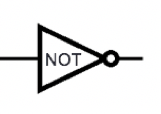
\includegraphics[height=0.5in]{../../resources/images/NOTx.png} \end{center}
\end{multicols}
% \begin{center}
%     \begin{tabular}{p{2in}p{2in}p{2in}}
%     \begin{center}\begin{tabular}{cc|c}
%     Inputs &  & Output \\
%     $x$ & $y$ & $x \text{ AND } y$  \\
%     \hline
%     $1$ & $1$ & $1$\\
%     $1$ & $0$ & $0$\\
%     $0$ & $1$ & $0$\\
%     $0$ & $0$ & $0$\\
%     \end{tabular}\end{center}
%     &
%     \begin{center}\begin{tabular}{cc|c}
%     Inputs &  & Output \\
%     $x$ & $y$ & $x \text{ XOR } y$  \\
%     \hline
%     $1$ & $1$ & $0$\\
%     $1$ & $0$ & $1$\\
%     $0$ & $1$ & $1$\\
%     $0$ & $0$ & $0$\\
%     \end{tabular}\end{center}
%     &
%     \begin{center}\begin{tabular}{c|c}
%     Input  & Output \\
%     $x$ & $\text{NOT } x$  \\
%     \hline
%     $1$ & $0$\\
%     $0$ & $1$\\
%     \end{tabular}\end{center}
%     \\
%     \begin{center}\includegraphics[height=0.6in]{../../resources/images/xANDy.png} \end{center} & 
%     \begin{center}\includegraphics[height=0.4in]{../../resources/images/xXORy.png} \end{center}& 
%     \begin{center}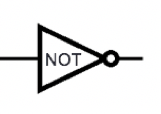
\includegraphics[height=0.5in]{../../resources/images/NOTx.png} \end{center}
%     \end{tabular}
%     \end{center}
A relation is a {\bf partial ordering} (or partial order) means 
it is reflexive, antisymmetric, and transitive.
A {\bf partition} of a set $A$ is a set of non-empty, disjoint subsets 
$A_1, A_2, \cdots, A_n$ such that 
\[
    A = \bigcup_{i=1}^{n} A_i = \{ x \mid \exists i (x \in A_i) \}
\]
{\bf  Definition}: A  {\bf predicate}  is  a function from a given set (domain) to $\{T,F\}$.
A predicate can be applied, or {\bf evaluated} at, an element of the domain.
Usually, a predicate {\it describes a  property} that domain elements may or may not have.
Two predicates over the same domain are {\bf equivalent} means they evaluate to
the same truth values for all possible assignments of domain elements to the
input. In other words, they are equivalent means that they are equal as functions.
To define a predicate, we must specify its domain and its value at each domain element.
The rule assigning truth values to domain elements can be specified using a formula, 
English description, in a table (if the domain is finite), or recursively (if the domain is recursively
defined).
{\bf Definition}: The {\bf truth  set} of a  predicate is the collection of all elements in its
domain where the predicate evaluates to $T$.
Notice that specifying the domain and the truth set is sufficient for defining
a predicate.
{\bf Definition}:  An integer $p$ greater than $1$ is called {\bf prime} means 
the only positive factors of 
$p$ are $1$ and $p$. A positive integer that is greater than $1$ and is not prime 
is called composite.
The {\bf universal quantification} of predicate $P(x)$ over
domain $U$ is the statement ``$P(x)$ for all values of $x$ in the domain $U$''
and is written $\forall x P(x)$ or $\forall x \in U ~P(x)$. 
When the domain is finite, universal quantification over the domain 
is equivalent to iterated {\it conjunction} (ands).
The {\bf existential quantification} of predicate $P(x)$ 
over domain $U$ is the statement ``There exists an element $x$ 
in the domain $U$ such that $P(x)$'' and is written $\exists x P(x)$
for $\exists x \in U ~P(x)$. 
When the domain is finite, existential quantification over the domain 
is equivalent to iterated {\it disjunction} (ors).
An element for which $P(x) = F$ is called a {\bf counterexample} of $\forall x P(x)$.
An element for which $P(x) = T$ is called a {\bf witness} of $\exists x P(x)$.

Colors can be described as amounts of red, green, and blue mixed together\footnote{This RGB representation
is common in web applications.  Many online tools are available to play around with mixing these colors, 
e.g. \url{https://www.w3schools.com/colors/colors_rgb.asp}. }
Mathematically, a color can be represented as a $3$-tuple $(r, g, b)$ where $r$
represents the red component, $g$ the green component, $b$ the blue component and where each of $r$, $g$, $b$ must
be a value from this collection of numbers:
\begin{quote}
$\{$0, 1, 2, 3, 4, 5, 6, 7, 8, 9, 10, 11, 12, 13, 14, 15, 16, 17, 18, 19, 20, 21, 22, 23, 24, 25, 26, 27, 28, 29, 30, 31, 32, 33, 34, 35, 36, 37, 38, 39, 40, 41, 42, 43, 44, 45, 46, 47, 48, 49, 50, 51, 52, 53, 54, 55, 56, 57, 58, 59, 60, 61, 62, 63, 64, 65, 66, 67, 68, 69, 70, 71, 72, 73, 74, 75, 76, 77, 78, 79, 80, 81, 82, 83, 84, 85, 86, 87, 88, 89, 90, 91, 92, 93, 94, 95, 96, 97, 98, 99, 100, 101, 102, 103, 104, 105, 106, 107, 108, 109, 110, 111, 112, 113, 114, 115, 116, 117, 118, 119, 120, 121, 122, 123, 124, 125, 126, 127, 128, 129, 130, 131, 132, 133, 134, 135, 136, 137, 138, 139, 140, 141, 142, 143, 144, 145, 146, 147, 148, 149, 150, 151, 152, 153, 154, 155, 156, 157, 158, 159, 160, 161, 162, 163, 164, 165, 166, 167, 168, 169, 170, 171, 172, 173, 174, 175, 176, 177, 178, 179, 180, 181, 182, 183, 184, 185, 186, 187, 188, 189, 190, 191, 192, 193, 194, 195, 196, 197, 198, 199, 200, 201, 202, 203, 204, 205, 206, 207, 208, 209, 210, 211, 212, 213, 214, 215, 216, 217, 218, 219, 220, 221, 222, 223, 224, 225, 226, 227, 228, 229, 230, 231, 232, 233, 234, 235, 236, 237, 238, 239, 240, 241, 242, 243, 244, 245, 246, 247, 248, 249, 250, 251, 252, 253, 254, 255$\}$
\end{quote}
\begin{enumerate}
\item \textbf{True} or \textbf{False}: $(1, 3, 4)$ fits the definition of a color above.
\item \textbf{True} or \textbf{False}: $(1, 100, 200, 0)$ fits the definition of a color above.
\item \textbf{True} or \textbf{False}: $(510, 255)$ fits the definition of a color above.
\item \textbf{True} or \textbf{False}: There is a color $(r_1, g_1, b_1)$ where $r_1 + g_1 + b_1$ is greater than $765$.
\item \textbf{True} or \textbf{False}: There is a color $(r_2, g_2, b_2)$ where $r_2 + g_2 + b_2$ is equal to $1$.
\item \textbf{True} or \textbf{False}: Another way to write the collection of allowed values for red, green, and blue components is $$\{x \in \mathbb{N}\mid 0 \leq x \leq 255 \}$$.
\item \textbf{True} or \textbf{False}: Another way to write the collection of allowed values for red, green, and blue components is $$\{n \in \mathbb{Z}\mid 0 \leq n \leq 255 \}$$.
\item \textbf{True} or \textbf{False}: Another way to write the collection of allowed values for red, green, and blue components is $$\{y \in \mathbb{Z}\mid -1 < y \leq 255 \}$$.
\end{enumerate}
\vfill
Recall the definition of linked lists from class.
Consider this (incomplete) definition:
{\bf Definition} The function $\textit{increment} : \underline{\hspace{6em}}$ 
that adds 1 to the data in each node of a linked list is defined by:
\[
\begin{array}{llll}
& & \textit{increment} : \underline{\hspace{3em}} & \to \underline{\hspace{3em}} \\
\textrm{Basis Step:} & & \textit{increment}([]) & = [] \\
\textrm{Recursive Step:} & \textrm{If } l \in L, n \in \mathbb{N} & \textit{increment}((n, l)) & = (1 + n, \textit{increment}(l))
\end{array}
\]
Consider this (incomplete) definition:
{\bf Definition} The function $\textit{sum} : L \to \mathbb{N}$ that adds 
together all the data in nodes of the list is defined by:
\[
\begin{array}{llll}
& & \textit{sum} : L & \to \mathbb{N} \\
\textrm{Basis Step:} & & \textit{sum}([]) & = 0 \\
\textrm{Recursive Step:} & \textrm{If } l \in L, n \in \mathbb{N} & \textit{sum}((n, l)) & = \underline{\hspace{8em}}
\end{array}
\]
You will compute a sample function application and then fill in the 
blanks for the domain and codomain of each of these functions.
\begin{enumerate}
    \item Based on the definition, what is the result of $\textit{increment}((4, (2, (7, []))))$? Write your answer directly with no spaces.
    
    \item Which of the following describes the domain and codomain of \textit{increment}?
    
    \begin{multicols}{2}
    \begin{enumerate}
        \item The domain is $L$ and the codomain is $\mathbb{N}$
        \item The domain is $L$ and the codomain is $\mathbb{N} \times L$
        \item The domain is $L \times \mathbb{N}$ and the codomain is $L$
        \item The domain is $L \times \mathbb{N}$ and the codomain is $\mathbb{N}$
        \item The domain is $L$ and the codomain is $L$
        \item None of the above
    \end{enumerate}
    \end{multicols}
    
    \item Assuming we would like $sum((5, (6, [])))$ to evaluate to $11$ and $sum((3, (1, (8, []))))$ to evaluate to $12$, which of the following could be used to fill in the definition of the recursive case of \textit{sum}?
    
     \begin{multicols}{2}
    \begin{enumerate}
        \item $\begin{cases}
            1 + \textit{sum}(l) & \textrm{when } n \neq 0 \\
            \textit{sum}(l) & \textrm{when } n = 0 \\
        \end{cases}$
        \item $1 + \textit{sum}(l)$
        \item $n + \textit{increment}(l)$
        \item $n + \textit{sum}(l)$
        \item None of the above
    \end{enumerate}
    \end{multicols}
    
    \newpage
    \item Choose only and all of the following statements that are \textbf{well-defined}; that is, they correctly reflect the domains and codomains of the functions and quantifiers, and respect the notational conventions we use in this class. Note that a well-defined statement may be true or false.
    \begin{multicols}{2}    
    \begin{enumerate}
        \item $\forall l \in L \, (\textit{sum}(l))$
        \item $\exists l \in L \, (\textit{sum}(l) \land \textit{length}(l))$
        \item $\forall l \in L \, (\textit{sum}(\textit{increment}(l)) = 10)$
        \item $\exists l \in L \, (\textit{sum}(\textit{increment}(l)) = 10)$
        \item $\forall l \in L \, \forall n \in \mathbb{N} \, ((n \times l) \subseteq L)$
        \item $\forall l_1 \in L \, \exists l_2 \in L \, (\textit{increment}(\textit{sum}(l_1)) = l_2)$
        \item $\forall l \in L \, (\textit{length}(\textit{increment}(l)) = \textit{length}(l))$
    \end{enumerate}
    \end{multicols}
    
    \item Choose only and all of the statements in the previous part that are both well-defined and true.
\end{enumerate}
Which of the following formalizes the definition of the predicate
$Pr(x)$ over the set of integers, and evaluates to $T$ exactly when 
$x$ is prime. (Select all and only correct options.)
\begin{enumerate}
    \item $\forall a \in \mathbb{Z}^{\neq 0}~( ~(x > 1 \land a >0) \to F(~(a,x)~))$
    \item $\lnot \exists a \in \mathbb{Z}^{\neq 0} ~(x > 1 \land (a=1 \lor a=x) \land F(~(a,x)~))$
    \item $(x > 1) \land \forall a \in \mathbb{Z}^{\neq 0}~( ~(~ a>0 \land F(~(a,x)~)~) \to (a=1 \lor a=x)~)$
    \item $(x > 1) \land \forall a \in \mathbb{Z}^{\neq 0}~( ~(~ a>1 \land \lnot (a=x) ~) \to \lnot F(~(a,x)~)~)$
\end{enumerate}
Which of the following are (recursive) definitions of the set of integers $\mathbb{Z}$?
(Select True/False for each one.)
\begin{enumerate}
\item 
\[
\begin{array}{ll}
\textrm{Basis Step: } & 5 \in \mathbb{Z} \\
\textrm{Recursive Step: } & \textrm{If } x \in \mathbb{Z} \textrm{, then } x+1 \in \mathbb{Z}
\textrm{ and } x-1 \in \mathbb{Z}
\end{array}
\]
\item 
\[
\begin{array}{ll}
\textrm{Basis Step: } & 0 \in \mathbb{Z} \\
\textrm{Recursive Step: } & \textrm{If } x \in \mathbb{Z} \textrm{, then } x+1 \in \mathbb{Z}
\textrm{ and } x-1 \in \mathbb{Z} \textrm{ and } x+2 \in \mathbb{Z} \textrm{ and } x-2 \in \mathbb{Z}
\end{array}
\]
\item 
\[
\begin{array}{ll}
\textrm{Basis Step: } & 0 \in \mathbb{Z} \\
\textrm{Recursive Step: } & \textrm{If } x \in \mathbb{Z} \textrm{, then } x+2 \in \mathbb{Z}
\textrm{ and } x-1 \in \mathbb{Z}
\end{array}
\]
\item 
\[
\begin{array}{ll}
\textrm{Basis Step: } & 0 \in \mathbb{Z} \\
\textrm{Recursive Step: } & \textrm{If } x \in \mathbb{Z} \textrm{, then } x+1 \in \mathbb{Z}
\textrm{ and } x+2 \in \mathbb{Z}
\end{array}
\]
\end{enumerate}
The {\bf set  of rational numbers}, $\mathbb{Q}$  is defined as 
\[
\left\{ \frac{p}{q} \mid p \in \mathbb{Z}  \text{ and  } q  \in \mathbb{Z} \text{ and } q \neq  0 \right\}
\text{~~~~or, equivalently,~~~~}
\{ x  \in  \mathbb{R} \mid \exists p \in \mathbb{Z}  \exists q \in \mathbb{Z}^+ ( p =  x \cdot q) \}
\]
{\it Extra practice}: Use the definition of set equality to prove that the definitions above  give the same set.


A relation $R$ on a set $A$ is called {\bf reflexive} 
means $(a, a) \in R$ for every element $a \in A$. 

{\it Recall the definitions}: The set of RNA strands $S$ is defined (recursively) by:
\[
\begin{array}{ll}
\textrm{Basis Step: } & \A \in S, \C \in S, \U \in S, \G \in S \\
\textrm{Recursive Step: } & \textrm{If } s \in S\textrm{ and }b \in B \textrm{, then }sb \in S
\end{array}
\]
where $sb$ is string concatenation.
The function \textit{rnalen} that computes the length of RNA strands in $S$ is defined recursively by:
\[
\begin{array}{llll}
& & \textit{rnalen} : S & \to \mathbb{Z}^+ \\
\textrm{Basis Step:} & \textrm{If } b \in B\textrm{ then } & \textit{rnalen}(b) & = 1 \\
\textrm{Recursive Step:} & \textrm{If } s \in S\textrm{ and }b \in B\textrm{, then  } & \textit{rnalen}(sb) & = 1 + \textit{rnalen}(s)
\end{array}
\]
The function \textit{basecount} that computes the number of a given base 
$b$ appearing in a RNA strand $s$ is defined recursively by:
\[
\begin{array}{llll}
& & \textit{basecount} : S \times B & \to \mathbb{N} \\
\textrm{Basis Step:} &  \textrm{If } b_1 \in B, b_2 \in B & \textit{basecount}(~(b_1, b_2)~) & =
        \begin{cases}
            1 & \textrm{when } b_1 = b_2 \\
            0 & \textrm{when } b_1 \neq b_2 \\
        \end{cases} \\
\textrm{Recursive Step:} & \textrm{If } s \in S, b_1 \in B, b_2 \in B &\textit{basecount}(~(s b_1, b_2)~) & =
        \begin{cases}
            1 + \textit{basecount}(~(s, b_2)~) & \textrm{when } b_1 = b_2 \\
            \textit{basecount}(~(s, b_2)~) & \textrm{when } b_1 \neq b_2 \\
        \end{cases}
\end{array}
\]
{\bf New! Recursive Definitions of Sets}: The set $S$ (pick a name) is defined by:
\[
\begin{array}{ll}
\textrm{Basis Step: } & \textrm{Specify finitely many elements of } S\\
\textrm{Recursive Step: } & \textrm{Give rule(s) for creating a new element of } S \textrm{ from known values existing in } S, \\
& \textrm{and potentially other values}. \\
\end{array}
\]
The set $S$ then consists of all and only elements that are put in $S$ by finitely many (a nonnegative integer number) of
applications of the recursive step after the basis step.
{\bf Definitions}:
A {\bf set} is an  unordered collection of  elements.
When $A$ and  $B$ are sets,  $A = B$ (set equality) means  
\[
    \forall x  ( x\in A \leftrightarrow x \in B)
\]
When $A$ and  $B$ are sets, $A \subseteq B$ (``$A$ is a {\bf subset} of $B$") means 
\[
    \forall x  (x \in A  \to x  \in B)
\]
When $A$ and  $B$ are sets,  $A \subsetneq B$ (``$A$ is a {\bf proper subset} of $B$") means 
\[
    (A\subseteq B) \wedge  (A \neq B)
\]
{\bf Definition}: A function $f: D  \to C$ is {\bf onto} (or  surjective) means for every $b$ in the codomain, 
there  is an element $a$ in the domain with  $f(a) = b$.
Formally, $f: D  \to  C$ is  onto  means $\underline{\phantom{\forall b \in C  \exists a \in D ( f(a) = b)}}$.

A relation $R$ on a set $A$ is called {\bf symmetric} means 
$(b, a) \in R$ whenever $(a, b) \in R$, for all $a, b \in A$. 

A relation $R$ on a set $A$ is called {\bf transitive} means 
whenever $(a, b) \in R$ and $(b, c) \in R$, then $(a, c) \in R$, for all $a, b, c \in A$.


\end{document}